\section{Evaluation}
\label{sec:evaluation}

We analyze over 3,000,000 SCOPE jobs over a period of five days that run on five data centers at Microsoft. 
In summary, our experiments answer the following questions:

\begin{itemize}
\item \emph{What is the proportion of time spent in native vs. non-native job vertices?}
Between \nonNativeTimeL{} and \nonNativeTimeU \% of data center time is spent in job vertices that run managed code.

\item \emph{What proportion of time can be optimized by inlining UDFs using  the current list of intrinsics?} 
Given the set of UDFs we found in our survey and  the current list of intrinsics we can optimize up to \optimizableU{} \% of data center time.

\item \emph{What proportion of time can be optimized by extending the list intrinsics? 
Which methods should be the most important for C++ implementation?}
By increasing the list of intrinsics and optimizing all inlineable methods we can optimize up to \potentiallyOptimizableU{} \% of data center time. 
Furthermore, we conclude that \emph{String} methods are the most important .NET framework methods amenable for C++ implementations.


\end{itemize}

\subsection{Experimental Setup}
To understand performance bottlenecks in SCOPE jobs we analyze over 3,000,000 jobs across 5 data centers.
Table~\ref{tb:projects} lists, for each data center, the number of analyzed jobs along with their CPU time measured in hours.
We observe that number of jobs and CPU time significantly vary between data centers. 
For example, data center \emph{cosmos15} run the highest proportion of jobs we analyze, while \emph{cosmos9} run the most expensive jobs. 
This is expected because different data centers are usually tailored for different types of jobs. 


\begin{table}[ht]
\centering
\begin{tabular}{lrr}
  Data center & Number of jobs & CPU time (in hours) \\
 \midrule
cosmos8 & 375,974 &  28,559,063 \\
cosmos9 & 171,203 &  40,714,052 \\
cosmos11 & 851,222 & 23,312,271\\
cosmos14 & 474,911 & 21,299,039\\
cosmos15 & 1,200,026&31,324,407 \\
\midrule
Total: & 3,073,336 & 145,208,834\\
\midrule
\end{tabular}
 \caption{Analyzed jobs and their CPU time
\label{tb:projects}}
\end{table}

The table shows that the jobs take a significant amount of resources. 
While we do not have access to the actual cost of these jobs, a very conservative estimate is to use $0.6$ cents an hour, the cost of the cheapest Amazon EC2 instance~\footnote{as of August 2017} at the time of writing. 
Given that most of these jobs run recurrently every day (some every hour), extrapolating these costs amounts to over $650$ million dollars per year. 
Thus, even a $1$\% performance improvement on these jobs will result in significant performance savings. 


\subsection{Native vs. Non-Native Time}
\begin{figure*}[ht]
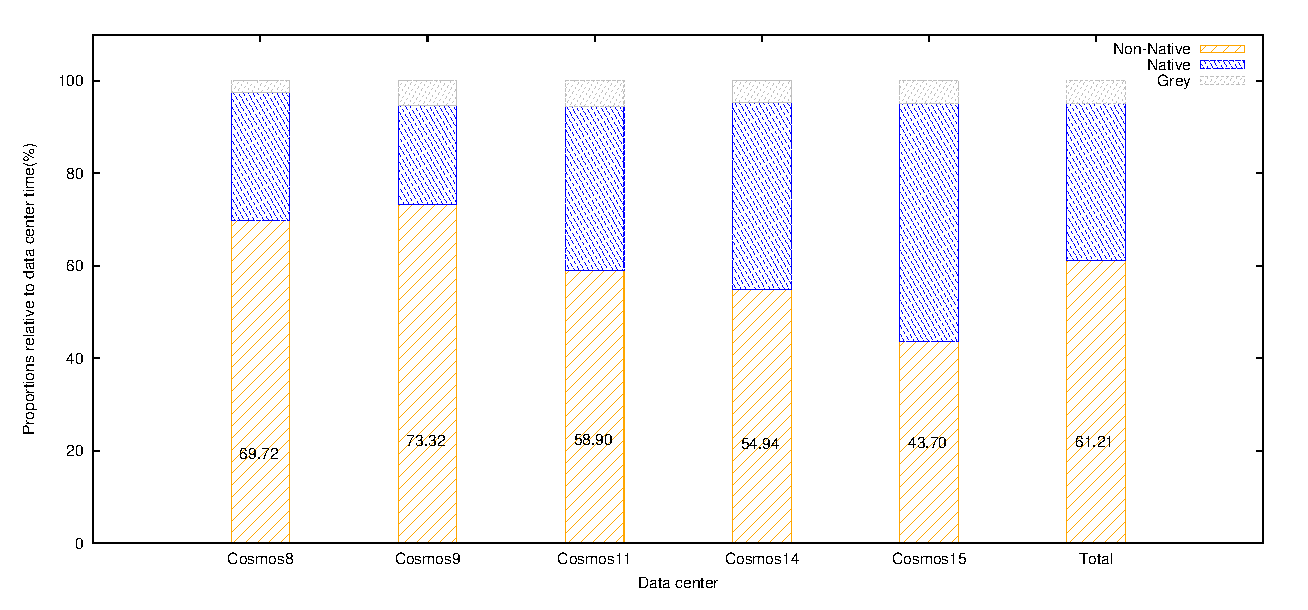
\includegraphics[width=2\columnwidth]{graphs/proportions2}
\caption{Time spent in native vs. non-native vertices}
\label{fig:nativeVsNonNative}
\end{figure*}
The first goal of our analysis is to determine the amount of time spent between native and non-native vertices of SCOPE jobs. 
As mentioned in Section~\ref{sec:nativenonnative}, SCOPE runs all relational logic efficiently in native code, while user-defined non-relational code is run in the CLR. 
Apart from avoiding the inherent overheads of running in non-native mode, the relational logic has the additional advantage of using all of the traditional optimizations modern databases typically perform.
From prior analyses, it was known that around $80$\% of the SCOPE jobs  use only relational constructs and thus run purely natively. 
Thus, at the outset, it was not obvious that non-relational optimizations would provide overall datacenter performance improvements. 


%Before optimizing non-relational logic in SCOPE jobs, it is important to understand how much time is spent in job vertices that run non-relational code. 
%The analysis of C++ code returns for every job vertex whether it runs as native or managed code. 
%Combined with data from \emph{Runtime Statistics} we also find how much time is taken by every job vertex.

Figure~\ref{fig:nativeVsNonNative} shows for every data center the time spent executing native vertices versus non-native vertices. 
For this analysis, we combined the time taken by every job vertex from \emph{Runtime Statistics} with additional analysis of C++ code that determines whether each operator within a vertex is run in native or non-native mode. 
Our analysis of the C++ code is conservative and reports an operator as running in non-native mode only if the analysis is able to detect the source of the managed C\# code or managed dll. 
Due to this conservative analysis, we tag some vertices as gray if the job metadata claims to include non-native operators but we are unable to detect the source. 
Modulo bugs in the SCOPE job metadata, these gray vertices are likely to be non-native vertices. But without improving our analysis we are unable to confirm this. 

%much time is spent in native and non-native vertices. 
%Grey area denotes few exceptional vertices for which the analysis can not certainly distinguish the code that runs inside a vertex. 
%For example, sometimes the analysis does not detect any source of managed code in a vertex that supposedly runs C\# code. 
%The time of such vertices we assign to gray area.

Figure~\ref{fig:nativeVsNonNative} shows that the time spent in non-native vertices represents a large fraction of data center time, ranging from $43.7$\% for cosmos15 to $73.3$\% for cosmos9. 
We can derive many conclusions from these results. First, these results could reflect the fact that the decades of work in optimizing relational code has borne fruit --- purely relational components account for a smaller percentage of datacenter runtime. Second, it could very well be the case that jobs with inherently expensive computations require logic that does not fit within the relational subset of SCOPE, and thus requires the use of non-native code. Finally,
these results could reflect the inherent overheads of running non-native code in the context of big-data processing. 

We did preliminary experimentation on a small subset of the jobs locally to study the performance bottlenecks of SCOPE jobs with managed operators. 
Our profiles show that the presence non-relational components reduce the throughput of a job by a factor of $10\times$ or more, with the performance bottleneck being the serialization/deserialization overhead of converting data into and from C\# objects. Note that we are unable to run most of the jobs locally as accesses to the data they process is severely restricted due to privacy concerns. Thus, it is quite possible that the results from our preliminary experimentation might not be representative of the jobs that run on the datacenters. Nevertheless, conversations with the SCOPE team validated these experiments, and Figure~\ref{fig:nativeVsNonNative} shows the potential performance improvements possible by optimizing the interaction between native and non-native parts of SCOPE. 



%For example, in cosmos9, the time spent in native <vertices contributes to only 21.30\% of data center time. 
%T

\subsection{Optimizable Job Vertices}
We say a job vertex is \emph{optimizable} if its only source of managed code comes from inlineable methods that in turn have only calls to existing intrinsics. 
An example of such a job is shown in Figure~\ref{fig:example}.
This is an extremely conservative definition, but it allows us to quantify how much data center time we can optimize given the current list of intrinsics. 
Moreover, by inlining method calls, we expect an entire vertex to run as native code, which should significantly improve the vertex execution time.

Figure~\ref{fig:optimizable} shows the proportion of CPU time of \emph{optimizable} vertices relative to data center time and to time spent in vertices with non-native code. 
We observe that with the current list of intrinsics we can optimize a relatively small proportion of data center time. 
For example, in cosmos9 that runs the most expensive jobs, we can optimize at most 0.01\% of data center time. 
The situation is slightly better in cosmos14 and cosmos15, but in these data centers, the proportion of non-native time is relatively lower compared to cosmos9.

The crucial observation is that given results illustrate only the time in data centers that can be affected by inlining method calls in optimizable vertices. 
To measure the actual performance improvement it is necessary to rerun every optimized job. 
Further details on performance improvements for several jobs we optimize are given in Section~\ref{sec:caseStudy}.

\begin{figure}[ht]
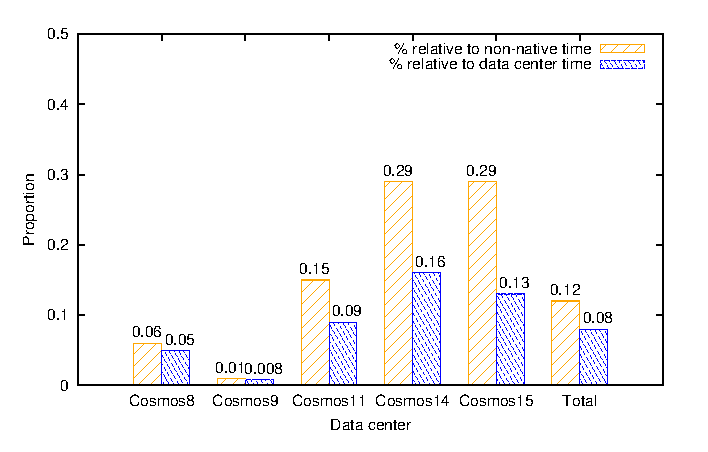
\includegraphics[width=\columnwidth]{graphs/optimizable2}
\caption{Optimizable job vertices}
\label{fig:optimizable}
\end{figure}

\subsection{Potential for C++ Translation}
To motivate the importance of providing the C++ implementation for more framework methods, we measure how much time is spent in the following type of vertices:
\begin{itemize}
\item Vertices with .NET framework calls as the only source of managed code
\item Vertices with .NET framework calls or calls to inlineable methods as the only source of managed code
\end{itemize}
We call these vertices \emph{potentially optimizable}, because they can run as native by increasing the list of intrinsics.

Figure~\ref{fig:potentially} shows the proportion of time spent in potentially optimizable vertices relative to data center time. 
We measure the proportions by assuming that all .NET framework methods have C++ implementation.
Results illustrate that we can optimize between \potentiallyOptimizableL{} and \potentiallyOptimizableU{} \% of data center time by just increasing the list of intrinsics. 
Even though \potentiallyOptimizableL{} \% of time spent in cosmos9 looks relatively low, it counts for almost 407,140 CPU hours for a period of several days. 
Knowing this type of impact motivates the future work on enabling more C++ translation of framework methods.

\begin{figure}[ht]
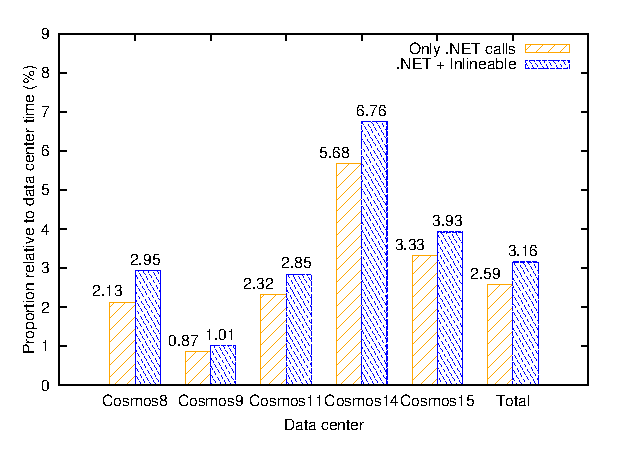
\includegraphics[scale=0.8]{graphs/potentiallyOptimizable}

\caption{Potentially optimizable job vertices}
\label{fig:potentially}
\end{figure}

\subsubsection{Most Relevant .NET Framework Methods}
Assuming that all .NET framework methods have C++ implementation is unrealistic. 
To provide more insights on the framework methods that actually matter, we perform two types of study:
the study of the most relevant methods considering the execution time of a vertex and the study of the most important method types. 

For the first study, we take all .NET framework methods called in potentially optimizable vertices and rank them based on the vertex execution time. 
Table~\ref{tb:rankedMethods} shows for every data center ten most important framework methods. 
The last row further illustrates how much data center time can be optimized if all methods in the list become intrinsics.
We further highlight methods that appear to be relevant across many data centers.
For example, \emph{System.String.ToLower} and \emph{System.String.Concat} are among the most relevant methods across all data centers.
Furthermore, if the native implementation is provided for the first ten methods in cosmos14, the data center it would be enough to optimize more than 5\% of data center time.

\begin{table*}[ht]
\small
 \begin{tabular}{@{}llllp{3.5cm}@{}}

  Cosmos8 & Cosmos9 & Cosmos11 & Cosmos14 & Cosmos15 \\
 \midrule
Convert.ToInt64 & \textbf{String.Equals} & String.Replace & \textbf{DateTime.ToString} & \textbf{String.ToLower} \\
Int32.Parse & \textbf{String.ToLower} & \textbf{String.ToLower} & String.IndexOf & String.LastIndexOf \\
\textbf{String.ToLower} & Int32.Parse & String.ToUpper & DateTime.ToLocalTime & \textbf{DateTime.ToString}\\
\textbf{String.Concat} & String.Replace & \textbf{String.Concat} & \textbf{String.ToLower} & \textbf{String.Concat}\\
String.Replace & Convert.ToDateTime & String.Trim & String.ToUpper & Convert.ToUInt64 \\
Double.Parse & Regex.isMatch & Math.Max & Regex.IsMatch & Enumerable.SelectMany \\
Math.Round& DateTime.ToUniversalTime & \textbf{String.Equals} & \textbf{String.Equals} & Enumerable.Distinct \\
Char.NewArr & \textbf{String.Concat} & TimeSpan.Days & \textbf{String.Concat} & String.Format \\
String.ToUpper & TimeSpan.Days & \textbf{DateTime.ToString} & String.Trim & \textbf{String.Equals}\\
String.Upper & DateTime.Subtract & String.ToCharArray & String.Split & String.IndexOf \\

\midrule
1.27\%\footnote{proportion relative to data center time} & 0.63\% & 1.61\% & 5.15\% & 1.8\%\\
\midrule

\end{tabular}
 
\caption{Most relevant .NET Framework methods per data center. All methods are within the {\tt System} namespace. Methods in bold are those that appear in the top 10 in at least 3 of the five data centers.
\label{tb:rankedMethods}}
\end{table*}


\begin{figure}[ht]
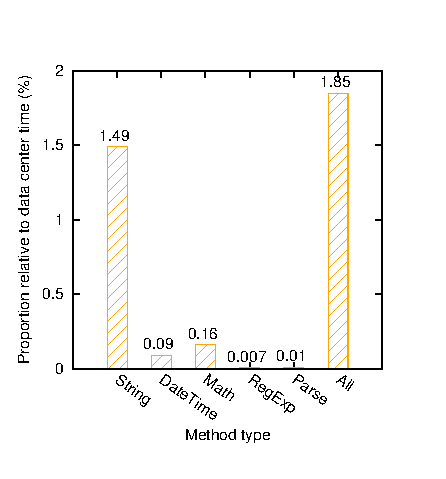
\includegraphics{graphs/methodTypes}
\caption{Relevance of .NET framework method types (cosmos11)}
\label{fig:methodTypes}
\end{figure}

Figure~\ref{fig:methodTypes} illustrates the most important method types for data center cosmos11. The results are comparable for other data centers. \emph{String} methods dominate and they count as the only source of non-native code in  1.49\% of the time spent in potentially optimizable vertices. Other method types are significantly less relevant, but when combined they influence 1.85\% of the data center time. These studies show the potential for improving data center performance by providing more intrinsics and thus enabling more C++ translation.






